\section{Presentazione della soluzione proposta (in termini generali)}

\begin{wrapfigure}{r}{.45\textwidth}
	\centering
	\vspace{-15mm}
	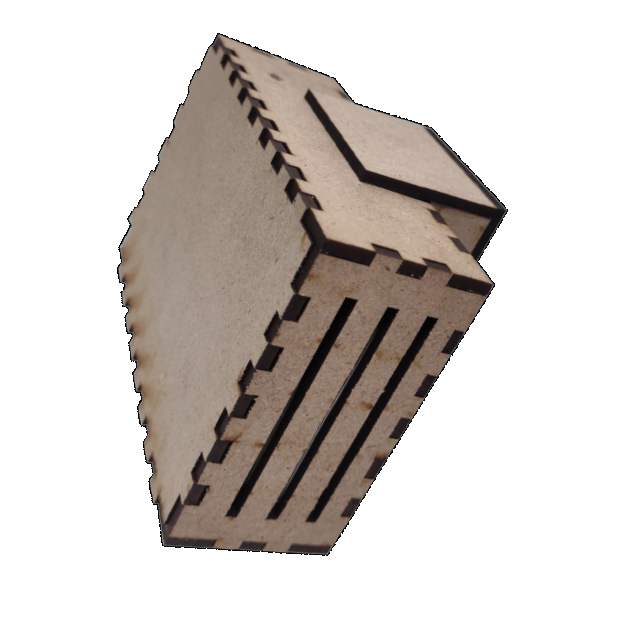
\includegraphics[width=.4\textwidth]{images/potnet.png}
	\vspace{-7mm}
	\caption{PotNet}
	\vspace{-5mm}
	\label{fig:potnet}
\end{wrapfigure}

\subsection{Descrizione generale}

La soluzione che proponiamo è \textbf{PotNet}, un \textbf{dispositivo intelligente che interagisce con l'utente e lo supporta durante il ciclo di vita della propria pianta}. In figura \ref{fig:potnet} è possibile vedere un primo prototipo che mostra il principale punto di forza di PotNet: l'\textbf{adattabilità}, a cui si uniscono il suo essere \textit{smart} e la sua facilità di utilizzo.

PotNet, infatti, si aggancia ai vasi comunemente presenti nelle abitazioni e, una volta configurato, grazie ai suoi numerosi sensori inizia a \textbf{monitorare e controllare i parametri vitali della pianta}.
Dopo averlo connesso ad internet, tramite la sua interfaccia web o grazie all'integrazione con Telegram, è necessario informare PotNet su quale sia il tipo di pianta presente nel vaso: inizierà così a monitorare la pianta e avviserà l'utente nel caso in cui uno o più parametri si discosti troppo dai valori ottimali.

Sarà sempre possibile richiedere lo stato della pianta o consigli su come migliorare il suo stato di salute tramite le numerose interfacce disponibili (assistente vocale, telegram, web UI). Inoltre, PotNet, invierà brevi report periodici per informare l'utente sull'andamento di salute della pianta.

\subsection{La regola del C$^3$}

\begin{figure}[h]
	\centering
	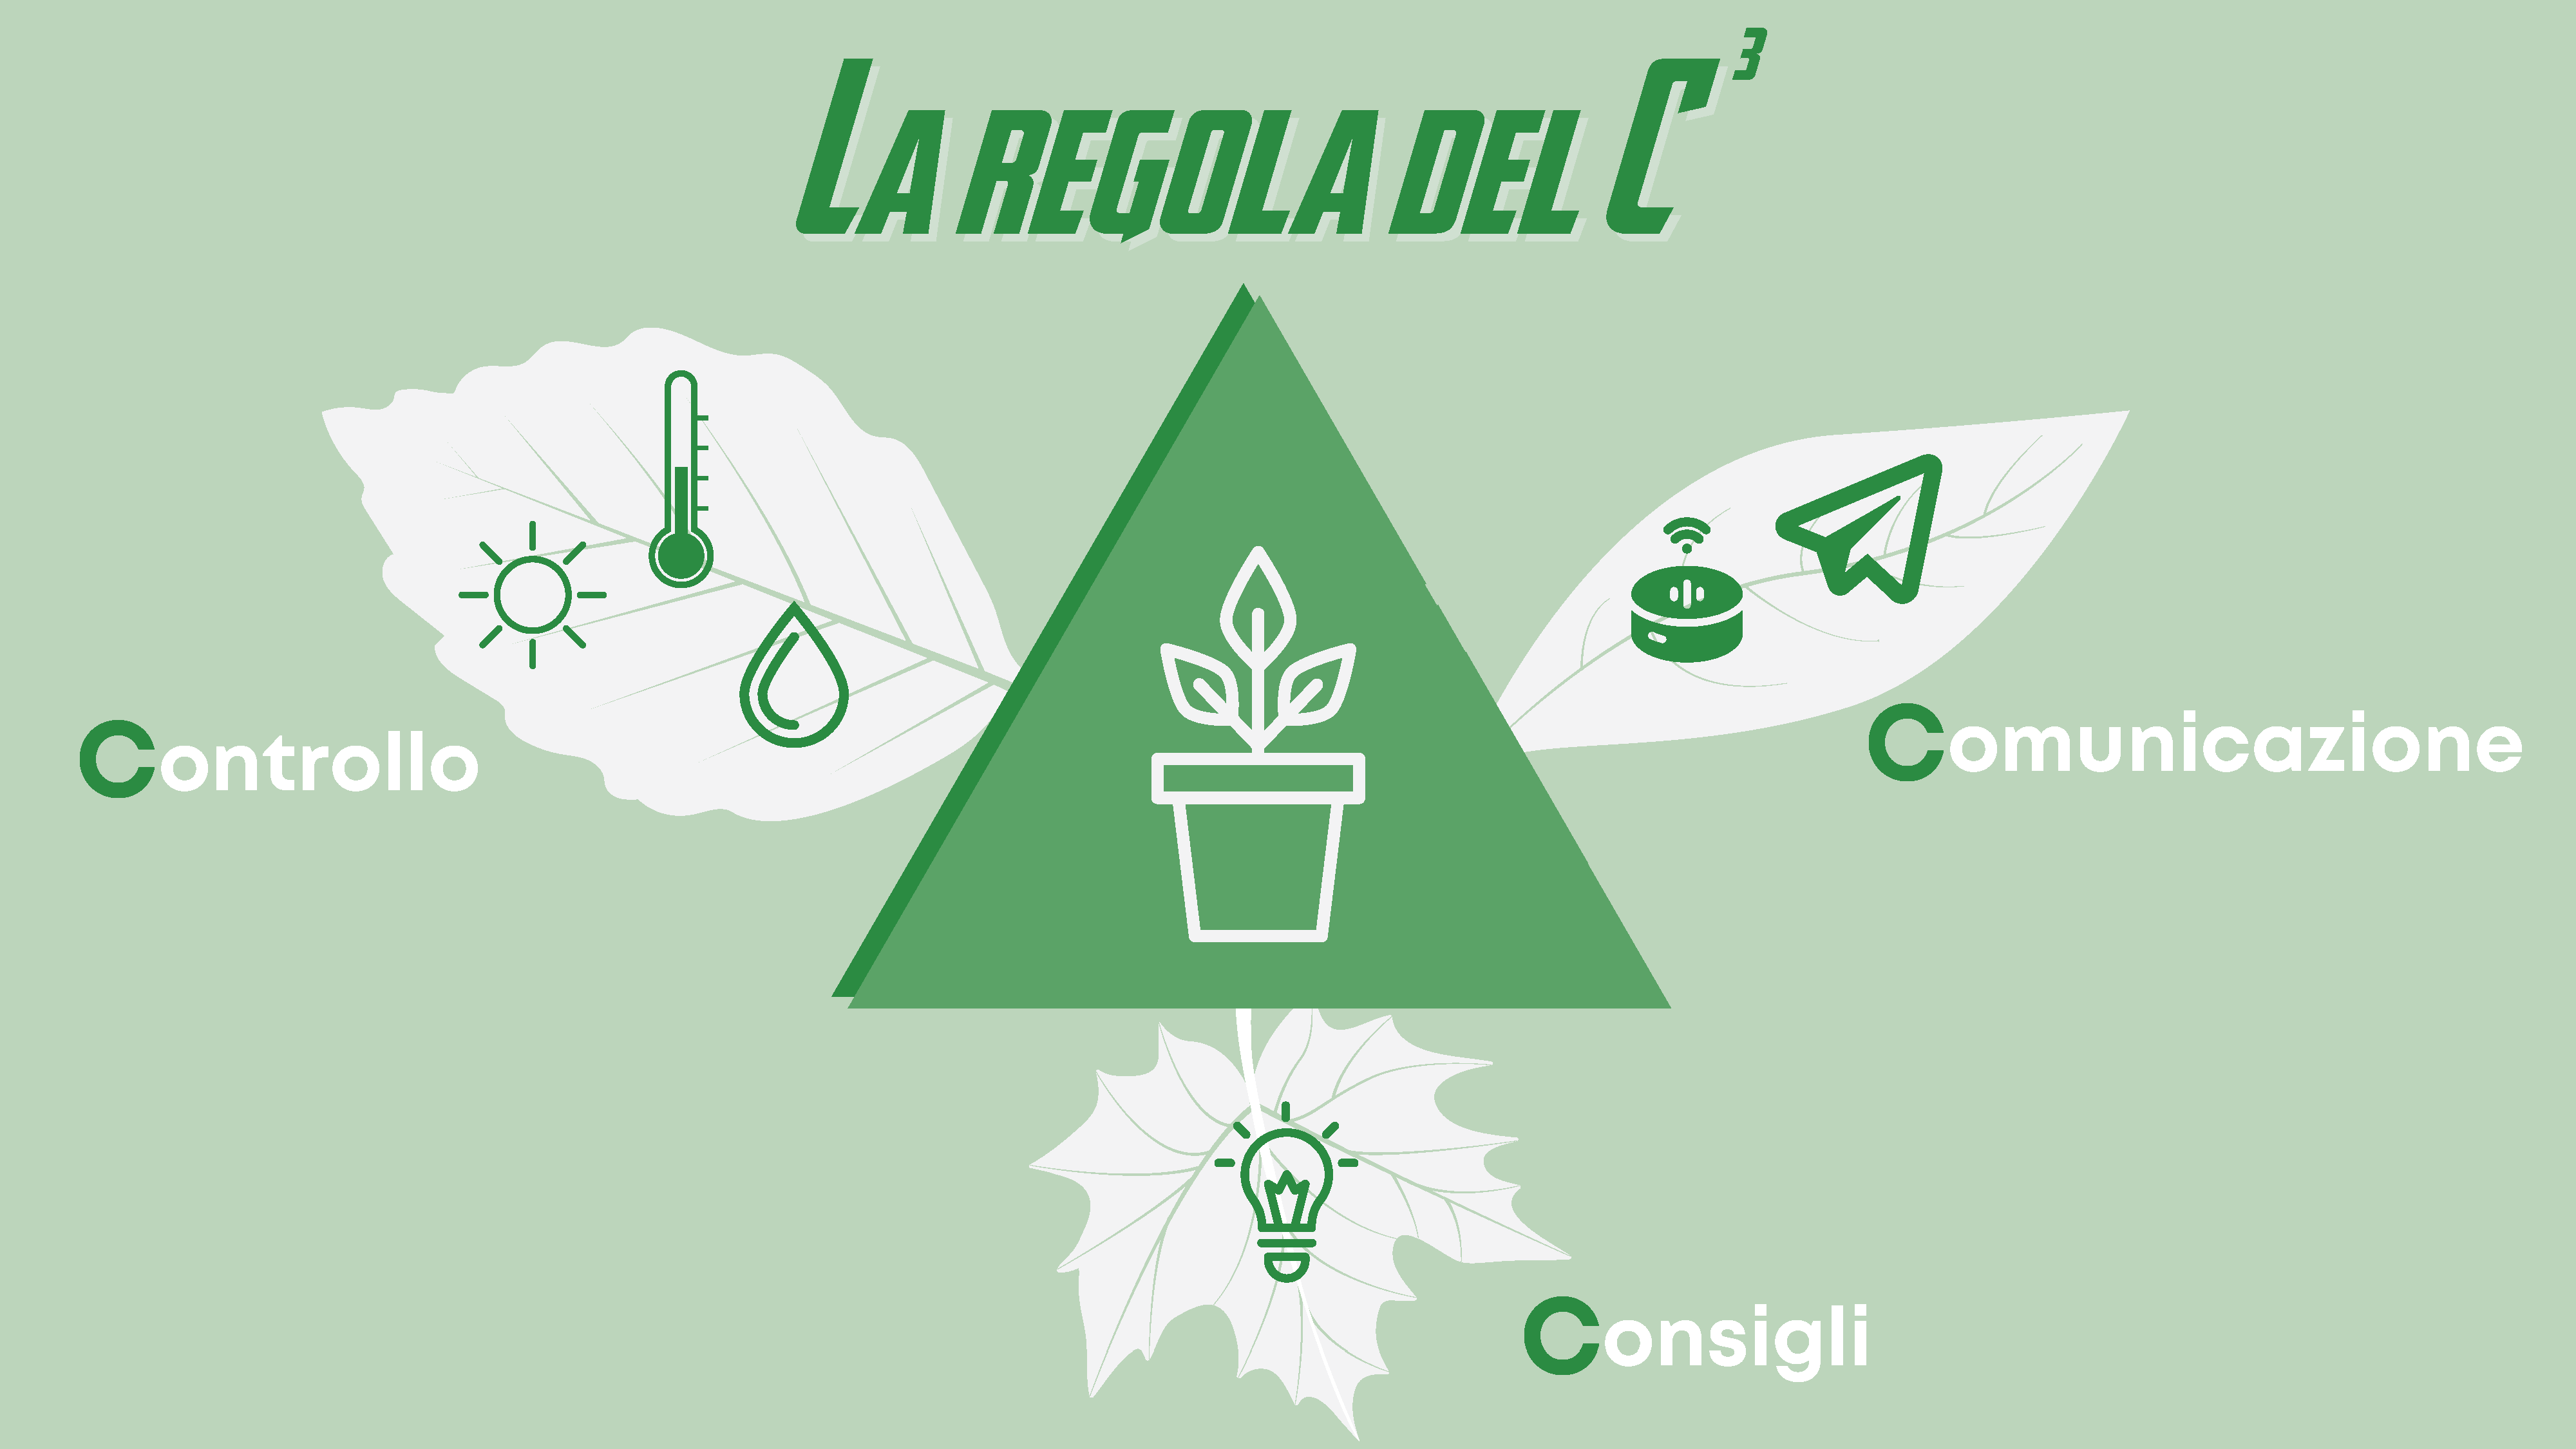
\includegraphics[width=.5\textwidth]{images/c3_rule.png}
	\caption{La regola del C$^3$}
	\label{fig:c3rule}
\end{figure}

PotNet segue la \textbf{regola del C$^3$}:
\begin{itemize}
	\item \textbf{Controllo}\\
	PotNet monitora continuamente tutti i parametri vitali della pianta e si accorge subito di qualche variazione o cambiamento significativo. Per ora, si controllano:
	\begin{itemize}
		\item \textit{temperatura e umidità} dell'ambiente che circonda la pianta;
		\item \textit{quantità di luce} che arriva alla pianta.
	\end{itemize}
	
	\item \textbf{Consigli}\\
	PotNet invia all'utente alcuni consigli personalizzati utili per far crescere correttamente la sua pianta.
	
	\item \textbf{Comunicazione}\\
	PotNet comunica con l'utente grazie a \textit{Telegram}, inviando immediatamente delle notifiche qualora sia richiesto il suo l'intervento (ad esempio quando la pianta è in un ambiente troppo freddo o troppo caldo). Inoltre, PotNet estende questo tipo di interazione integrandosi con gli assistenti vocali\footnote{Nella versione prototipale di PotNet è stata scelta Alexa, ma è prevista anche l'integrazione con l'assistente vocale \textit{Google}}.
\end{itemize}

\subsection{Proposizione di valore}

\begin{figure}[h]
	\centering
	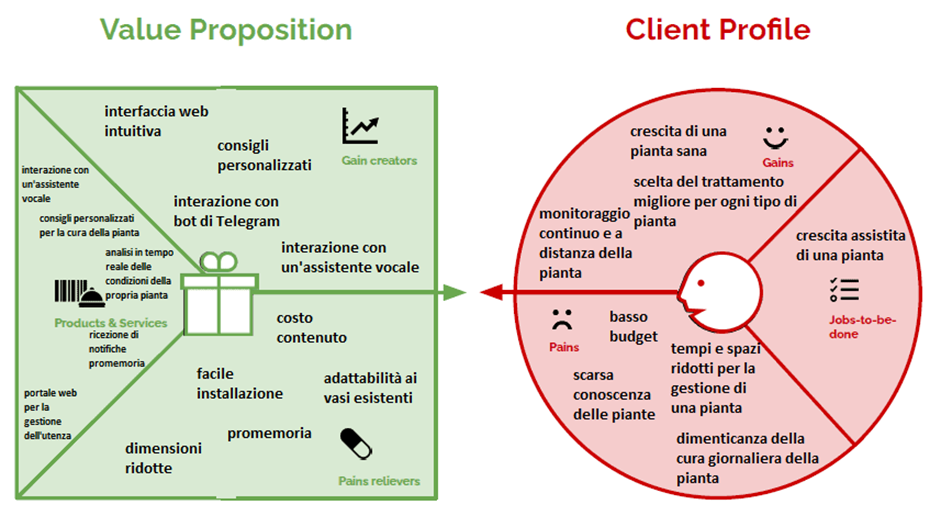
\includegraphics[width=\textwidth]{images/value_proposition.png}
	\caption{Canvas della proposizione di valore}
	\label{fig:value_proposition}
\end{figure}

La figura \ref{fig:value_proposition} mostra il \textit{canvas} della \textit{proposizione di valore} di PotNet.